% TODO - Ilk paragraf baglanacak 

\section{Introduction} \label{sec:intro}
%\subsection{Motivation}
% Think about a cat alone in darkness with a hungry stomach waiting for her owner.

Are cats only a means to joy for humans, or are they rather precious companions? It is easier to answer this question after a quick reminder of a historical event: In \(14^{th}\) century, Europe was swept over by a plague, mainly resulted by the bites of infected rats, lice and mice. People of Europe at the time were certain that this plague was God's punishment, so the `logical' reaction was to execute Jews and alleged witches. During this manhunt, some communities also massacred village cats, thinking they were associated with witches. The removal of cats from the equation allowed a crazy amount of infected rats to continue spreading the disease, which gave way to the infamous black death.
This is only one of many reasons why humans need to appreciate cats and take good care of them when necessary. Felerest, knowing that cats are not evil, believes the appreciation of human kind's precious companions should be built on solid ground.

% TODO - tamamlanmalı




%\subsection{Related Work}
The current autonomous cat feeding systems have only a few capabilities and are quite costly. The state of the art, according to an article on most rated automatic cat feeding systems of 2019 \cite{cite:SOTA}, has several key features. These are large food storage capacity, portion control settings, kibble size options and pet-proofing. This system costs 150 dollars. However, we intend to achieve all of this with extra capabilities with a maximum budget of 200 dollars. The proposed system will identify and recognize different cats and track their dietary plans. In addition to this, the proportions will be distributed with weights of the cats in mind. The system will be capable of feeding a large number of cats making it adoptable for usage in campuses and homes where cats are handful. The system's reservoir will be adequate to feed more than 20 cats for the duration of the battery lifetime, 10 hours.

There are various parameters involving a cat's appetite like its age, gender, weight, environmental factors and the brand of cat food. When the brand changes, the kcal per kg, kibble  size, volume per gram also change. Therefore, the calculations were held under many assumptions and idealizations. An average cat weighing 4kg needs to consume approximately 253 kcal/day \cite{cite:DIET}. This corresponds to an average of 60 grams of dry cat food per day. For a 10 hour span the food consumption per cat is 25grams which is nearly 50ml in volume. As the reservoir volume is anticipated to be 5 liters, as many as 100 cats can be fed. 

%\st{Since there were many assumptions as mentioned these numbers have are not as realistic. However, the conclusion can be made that the designed system can easily achieve the system's goals.}{\color{red} WHAT}

%{\color{red} Should this paragraph really be here? Don't we have to just talk about current solutions?}{\color{blue} bence de bu yanlış yerde yazılmış}{\color{green} iste bana da oyle geldi yani} {\color{yellow}acik renk kullanmayin okuyamiyorum}{\color{Apricot} hakli isyan}

%\subsection{Societal Impact}
Societal marketing is one of the main concepts in the sustainable marketing environment. Companies have been developing techniques to create a sustainable world by putting some regulations into practice. Marketing has advanced such that society now has stronger impact on the market. Figure \ref{fig:intro_societalMarketing} shows the balance between company-customer-society where Felerest aims to create a sustainable and social environment \cite{bib:intro_societalMarketing}.


\begin{wrapfigure}{r}{0.5\textwidth}
    \centering
    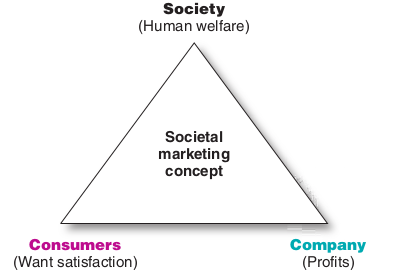
\includegraphics[width=0.4\textwidth]{img/intro_societalMarketingTriangle.png}
    \caption{\scriptsize Three Considerations in Societal Marketing \cite{bib:intro_societalMarketing}}
    \label{fig:intro_societalMarketing}
\end{wrapfigure}

Felerest also aims to be an environmentally friendly company that reduces trash, leftover, health risks, and energy consumption. The design allows users to easily replace broken parts by simply breaking down into sub-systems which diminishes the trash generated in repair phase and makes it impossible to impose planned obsolescence. Moreover, the regulated food drop mechanism not only provides a healthy diet that prevents cats from getting or staying overweight, but it also makes sure no food is wasted. In addition to these environmental effects, it consumes only a little power to run continuously, playing a part in reducing $CO_2$ emission and keeping the world sustainable. Felerest is ready to prove that it feels responsible for the environment, society, and future generations.

This report includes organization of the company, brief explanations about members, requirement analysis of the project, solution approaches to problems and expected deliverables of the project. 

%\st{Finally, protecting the environment and creating a sustainable world plays an important role in Felerest group because Felerest feels it is responsible for the society and the future generations.} {\color{red} this needs to be revisited***}
